\documentclass[12pt, a4paper, oneside]{article}  
\usepackage{ucs}
\usepackage[utf8x]{inputenc} 
\usepackage[russian]{babel}
\usepackage{amsmath}
\usepackage{amssymb}
\usepackage{tikz}
\usepackage{xcolor}
\usepackage{listings}
\usepackage{color}
\usepackage{graphics}
\usepackage[hidelinks]{hyperref}  


\definecolor{dkgreen}{rgb}{0,0.6,0}
\definecolor{gray}{rgb}{0.5,0.5,0.5}
\definecolor{mauve}{rgb}{0.58,0,0.82}

\lstset{frame=tb,
	language=Python,
	aboveskip=3mm,
	belowskip=3mm,
	showstringspaces=false,
	columns=flexible,
	basicstyle={\small\ttfamily},
	numbers=none,
	numberstyle=\tiny\color{gray},
	keywordstyle=\color{blue},
	commentstyle=\color{dkgreen},
	stringstyle=\color{mauve},
	breaklines=true,
	breakatwhitespace=true,
	tabsize=3
}

\usepackage{geometry}
\geometry{a4paper,left=30mm,right=15mm,top=20mm,bottom=20mm}
\renewcommand{\baselinestretch}{1.5}
\hbadness=99999

\author{Цзыкай А.}

\begin{document}
\clearpage
	\thispagestyle{empty}
	\renewcommand{\baselinestretch}{0.9}
		\begin{center}\footnotesize
			ФЕДЕРАЛЬНОЕ ГОСУДАРСТВЕННОЕ БЮДЖЕТНОЕ ОБРАЗОВАТЕЛЬНОЕ\\ УЧРЕЖДЕНИЕ ВЫСШЕГО ОБРАЗОВАНИЯ\\
			«МОСКОВСКИЙ ГОСУДАРСТВЕННЫЙ УНИВЕРСИТЕТ имени М.В.ЛОМОНОСОВА»\\
			ФИЗИЧЕСКИЙ ФАКУЛЬТЕТ\\
			КАФЕДРА МАТЕМАТИЧЕСКОГО МОДЕЛИРОВАНИЯ И ИНФОРМАТИКИ
		\end{center}
	\hrulefill
	
	~\\
	\renewcommand{\baselinestretch}{1}
		\begin{center}\Large
			\textbf{Курсовая работа}
			
			~\\
			\LARGE\textbf{«Принятие инвестиционных решений в условиях неопределенности»}\\[300pt]
		\end{center}
	
	
		\begin{flushright}\renewcommand{\baselinestretch}{0.9}
			Выполнил:\\
			\textbf{Студент 217 гр. А. Цзыкай}
			
			~\\
			Научный руководитель:\\
			\textbf{к. ф.-м. н. А. В. Зубюк}
		\end{flushright}
		
		~\\
		\begin{center}
			\textbf{Москва\quad 2022}
		\end{center}

\newpage
	\pagestyle{plain}
	\setcounter{page}{1}
	\tableofcontents
	\setcounter{secnumdepth}{0}

\newpage
	\begin{center}
		\section{Введение}
	\end{center}

	Многие обратные задачи, возникающие при анализе данных физического эксперимента, экономических данных и др. являются некорректно поставленными. Эти некорректно поставленные обратные задачи, имеющее решение не единственно, или решение не непрерывно зависят от входных данных, можно решить с помощью имеющейся априорной информацией в виде мягких качественных ограничений.
	
	В настоящей работе рассматриваются практические применения некорректно поставленных обратных задач оценивания в области инвестиционных решений. Для решения таких задач широко используется метод регуляризации, однако в настоящей работе предпочтение отдается подходу с мягкими качественными ограничениями, основанном на понятия теории возможности профессора Ю. П. Пытьева \cite{1}. Даны постановки задач с мягкими качественными ограничениями и предложены численные методы их решения в линейном и нелинейном случаях. В линейном случае задачи сводятся к задачам линейного программирования. В нелинейном предложены метод доверительных областей их решения. \cite{2}\\
	
	\begin{itemize}
		\item \textbf{Цель работы}\\
		Использование известной априорной информации для установления мягких качественных ограничений в условиях некорректно поставленных задач, и реализация соответственными математическими методами в области инвестиционных решений.
	\end{itemize}
	
\newpage
	\section{Глава 1. Мягкие качественные ограничения}
		\subsection{1.1	 Обратная задача оценивания и некорректность её постановки}
			В различных предметных областях, существует общая зависимость между известными наблюдениями и полезными сигналами, подлежащим оценивание:
			\begin{equation}
				\label{eq1}
				\xi = Af + \nu
			\end{equation}
			где $A$ -- линейный оператор, действующий из $\mathcal{R}^n \to \mathcal{R}^m$, соответственно $f$ является вектором n-мерного Евклидова пространства $\mathcal{R}^n$, и $\xi$ является вектором m-мерного Евклидова пространства $\mathcal{R}^m$. $\mu$ -- случайная погрешность преобразования,принимающая в $\mathcal{R}^m$ и моделирующая аддитивный шум. Поставленна обратная задача схемой \eqref{eq1}, в которой требуется оценить полезный сигнал $f$ по наблюдению $\xi$.

			\subsubsection{1.1.1 Некорректность обратной задачи оценивания при отсутствии априорной информации}
				\textbf{Определение 1.} Задача называется корректно поставленной (по Адамару), если выполнены следующие условия:\\
				1) Решение этой задачи существует;\\ 
				2) Решение задачи единственно;\\
				3) Решение непрерывно зависит от входных параметров.
				
				Некорректность задачи оценивания сигнала f при отсутствии априорной информации о нём, т. е. когда оценка строится исключительно на основе наблюдения , может быть обусловлена двумя факторами \cite{2}:
				
				1) Вырожденность оператора $A$,когда его ядро содержит не только нулевой элемент: $ker(A) \ne \{0\}$.
				
					Действительно, при отсутствии какой-либо априорной информации о $f$, если $\hat{f_1}$ -- полученная оценка сигнала $f$ (оптимальная в некотором смысле), то $\hat{f} = \hat{f_1} + \hat{f_2}$ также является справедливой оценкой исходного сигнала $f$, где $\forall \hat{f_2} \in ker(A)$. Значит, настоящие задачи с вырожденным оператором, имеющие не единственное решение.
				
				2) Плохая обусловленность оператора $A$, когда оператора $A$ имеет большое число обусловленности ($cond(A)\gg 1$).
				
					При достаточно большом числе обусловленности, в зависимости от входных параметров решение может изменяться непредсказуемым образом. Это фактор показывает, что решение зависит от входных параметров не непрерывным образом.
				
			\subsubsection{1.1.2 Обычное ограничение и мягкое ограничение}
				В случае наличия различных факторов, обусловливающих некорректность обратной задачи оценивания – вырожденности и (или) плохой обусловленности оператора A , – оценка сигнала f может быть представлена в виде:
				\begin{equation}
					\label{eq2}
					\hat{f} = \hat{f_1} + \hat{f_2}
				\end{equation}
				где компонента $\hat{f_1}$ находится известными методами, а $\hat{f_2}$ может быть любой в пределах некоторого известного множества $\mathcal{L}_2$ (которым может быть ядро $ker(A)$ оператора $A$ или подпространство $ker(A)$). Таким образом, при отсутствии априорной информации все оценки:
				\begin{equation}
					\label{eq3}
					\hat{f}\in \mathcal{L}=\hat{f_1}+\mathcal{L}_2=\{\hat{f_1}+\hat{f_2} | \hat{f_2}\in\mathcal{L}_2\}
				\end{equation}
			
				Для уточнения оценки в пределах множества $\mathcal{L}$ \eqref{eq3} используем априорную информацию об оцениваемом сигнале f и, следовательно, его оценке ограничений $\hat{f}$, заданную в форме системы мягких ограничений:
				\begin{equation}
					\label{eq4}
					c_i(\hat{f}) \gtrsim 0,\quad i = 1,\dots,k,
				\end{equation}
				где $c_i$ -- функции из $\mathcal{L}\to\mathbb{R}$, $\gtrsim 0$ -- мягкое унарное отношение на числовой прямой $\mathbb{R}$, которое мы будем понимать, как «мягкую неотрицательность». Таким образом, ограничения \eqref{eq4} мы будем интерпретировать как «скорее всего, $c(\hat{f})$ неотрицательны» для всех $i = 1,\dots,k$.\\
				
		\subsection{1.2 Теория возможности}
			\subsubsection{1.2.1 Мягкое унарное ограничение}
				В предыдущем разделе мы использовали мягкое отношение $\gtrsim 0$ для определения системы мягких ограничений, теперь мы определим его понятие и исследуем его основные свойства.
				
				\textbf{Определение 2.} Пара ($2^X,\ge_\pi$) является мягким унарным отношением на $X$, где $\ge_\pi$ -- полный предпорядок на множестве 2X всех подмножеств множества X. \cite{2}
				\begin{itemize}
					\item Обычное унарное отношение на X –- подмножество множества X.\\
						$2^X$ –- множество всех обычных унарных отношений на X.\\
					\item Мягкое унарное отношение ($2^X,\ge_\pi$) является математической формализацией пожеланий относительно вида обычного унарного отношения на X. \\
					ввести на $2^X$ полный предпорядок $\ge_\pi$ и определяем насколько хорошо элементы $2^X$ соответствуют нашим пожеланиям.
				\end{itemize}
				
				Для понятия разницы между четким унарным отношением $c \ge 0$ и мягким унарным отношением $c \gtrsim 0$, сравним их подмножества на $\mathbb{R}$:\\
				Четкое унарное отношение $c \ge 0$ -- это четкое подмножество на $\mathbb{R}$.\\
				
				\begin{center}
					\begin{tikzpicture}
					\draw[->] (-1.5,0)--(4.5,0);
					\foreach \x in {0}\draw (\x,0.2)--(\x,0)node[below]{$\x$};
					\draw[fill=blue!10] (4,0)--(0,0)--(0,1)--(4,1);
					\node at (4.3,0.2){c};
				\end{tikzpicture}
				\end{center}
				Мягкое унарное отношение $c \gtrsim 0$ -- это плохое известное подмножество $\mathcal{R}_{\gtrsim0}$ на $\mathbb{R}$\\
				
				\begin{center}
					\begin{tikzpicture}
					\draw[->] (-1.5,0)--(4.5,0);
					\foreach \x in {0}\draw (\x,0.2)--(\x,0)node[below]{$\x$};
					\draw[fill=blue!10] (4,0)--(2,0)--(2,1)--(4,1);
					\draw[fill=blue!10] (-1.5,0)--(1,0)--(1,1)--(-1.5,1);
					\node at (4.3,0.2){c};
					\node at (6.3,0.2){$\mathcal{R}_1\quad \pi(\mathcal{R}_1)$};
				\end{tikzpicture}
				
				\begin{tikzpicture}
					\draw[->] (-1.5,0)--(4.5,0);
					\foreach \x in {0}\draw (\x,0.2)--(\x,0)node[below]{$\x$};
					\draw[fill=blue!10] (4,0)--(2.5,0)--(2.5,1)--(4,1);
					\draw[fill=blue!10] (-1,0)--(1.5,0)--(1.5,1)--(-1,1)--(-1,0);
					\node at (4.3,0.2){c};
					\node at (6.3,0.2){$\mathcal{R}_2\quad \pi(\mathcal{R}_2)$};
				\end{tikzpicture}
				
				\begin{tikzpicture}
					\draw[->] (-1.5,0)--(4.5,0);
					\foreach \x in {0}\draw (\x,0.2)--(\x,0)node[below]{$\x$};
					\draw[fill=blue!10] (4,0)--(2,0)--(2,1)--(4,1);
					\node at (4.3,0.2){c};
					\node at (6.3,0.2){$\mathcal{R}_3\quad \pi(\mathcal{R}_3)$};
				\end{tikzpicture}
				\end{center}
			
				Когда мы вычисляем полный предпорядок $\ge_\pi$, можно рассматривать функцию $\pi: 2^X\to [0,1]$. Она предназначена для количественной оценки различных обычных унарных отношений соответствия нашим желаниям: $\pi(R_1)\ge\pi(R_2)\Leftrightarrow R_1\ge_\pi R_2, R_i\in 2^X$. Очевидно, что значения функции $\pi$ монотонного задаются с точностью до строго преобразования отрезка [0,1] с неподвижными точками 0 и 1. Такой подход к заданию полного предпорядка на множестве всех доступных альтернатив лег в основу теории возможностей Ю.П. Пытьева \cite{2}, в которой функция $\pi$ названа \textit{распределением возможностей}.
				
				
				
				Согласно принципу транзитивности унарных отношений, можно легко доказать следующую теорему о распределении вероятностей \cite{2}:
				
				\textbf{Определение 3. (принцип транзитивности)} Мягким отношением $\gtrsim 0$ назовём мягкое унарное отношение на $\mathbb{R}$, для любых $x,y\in\mathbb{R}$ удовлетворяющее условию:
				\[x\ge y,y\gtrsim 0\Rightarrow x\gtrsim 0.\]
				
				\textbf{Теорема 1.} $\pi_{\gtrsim 0}(R)>0$, только если $R = [a,\infty)$ -- полупрямая.\\
				
				
				
				\begin{center}
					\begin{tikzpicture}
					\draw[->] (-1.5,0)--(4.5,0);
					\foreach \x in {0}\draw (\x,0.2)--(\x,0)node[below]{$\delta$};
					\foreach \x in {1.5}\draw (\x,0.2)--(\x,0)node[below]{$y$};
					\foreach \x in {3}\draw (\x,0.2)--(\x,0)node[below]{$x$};
					\draw[fill=blue!10] (4,0)--(0,0)--(0,1)--(4,1);
					\node at (4.3,0.2){R};
				\end{tikzpicture}
				\end{center}
			
			\subsubsection{1.2.2 Мера возможности}
				Согласно \cite{1} мерой возможности является функция
				\[\Pi(\varepsilon) = \sup_{R\in\varepsilon}\pi(R)\qquad\Pi:\mathcal{P}(2^X)\to[0,1]\]
				где $\mathcal{P}(2^X)$ -- множество всех подмножеств $2^X$ (алгебра событий).
				
				Функция мерой возможности удовлетворяют следующей доказанной теории:
				
				\textbf{Теорема 2.} Возможность $\mu(x) = \Pi_{\gtrsim 0}(\{x\gtrsim 0\})$ того,что $x\gtrsim 0$, -- монотонно неубывающая функция аргумента $x$.
				
				Значение функции $\mu(x)$ представляет собой возможность удовлетворения мягкого ограничения $x\gtrsim 0$, и что эта возможность не уменьшается с ростом x.\\
				
		\subsection{1.3 Система мягких ограничений}
			С практической точки зрения, исследуемая нами задача \eqref{eq4} -- это не одно мягкое ограничение, а их система, имеющая вид:
			\[
				\left\{
				\begin{array}{lr}
					c_1 \gtrsim 0\\
					c_2 \gtrsim 0\\
					\vdots\\
					c_k \gtrsim 0\\
				\end{array}
				\right.
			\]

			Для того чтобы получить возможность этой системы, необходимо доказать еще одну теорему:
			
			\textbf{Теорема 3.} Возможность одновременного выполнения системы мягких ограничений $x_i\gtrsim 0, i=1,\dots,k,$ равна:
			\begin{eqnarray}
				\Pi_{\gtrsim 0}(\bigcap_{i=1}^k \{x_i\gtrsim 0\}) &=& \sup\{\pi_{\gtrsim 0}(R) | x_i\in R, i = 1,\dots,k\}	\nonumber \\
																  &=& \sup\{\pi_{\gtrsim 0}([a,\infty)) | a\le x_i, i =1,\dots,k\} \nonumber \\
																  &=& \sup\{\pi_{\gtrsim 0}([a,\infty)) | a\le \min_{i=1,\dots,k} x\} \nonumber \\
																  &=& \mu \min_{i=1,\dots,k} x_i = \min_{i=1,\dots,k} \mu(x_i) \nonumber
			\end{eqnarray}
		
	\section{Глава 2. Реализация численных методов решения и практические применения}
		Возвращаясь к математической задаче поиска оценки $\hat{f}$ \eqref{eq1}, поставленной в начале нашей работой. В результате всего показанного в предыдущей главе, эту задачу можно поставить как поиска вектора $\hat{f}\in \mathcal{L}$, который максимизирует возможность одновременного выполнения системы мягких ограничений \eqref{eq4}, т.е. как оптимизационная задача $\min_{i=1,\dots,k}\mu(c_i\hat{f}) \sim \max_{\hat{f}\in\mathcal{L}}$, которая с учётом монотонности $\mu$ принимает вид:
			\begin{equation}
				\label{eq5}
				\min_{i=1,\dots,k}c_i(\hat{f}) \sim \max_{\hat{f}\in\mathcal{L}}
			\end{equation}
		
		В рассматриваемых обратных задачах оценивания, линейность оператора $A$ приводит к линейности множества $\mathcal{L}$ в \eqref{eq5}, затем в нем функции  $c_i$, задающие мягкие ограничения \eqref{eq4}, можно рассматривать в двух случаях: линейном и нелинейном.
			
		\subsection{2.1 Решения обратной задачи оценивания с линейными мягкими ограничениями}
			Если каждая из функций $c_i$ линейна, то задача \eqref{eq5} может быть сведена к задаче линейного программирования:
			\begin{equation}
				\label{eq6}
				z \sim \max_{\hat{f}\in\mathcal{L},z\in \mathbb{R}},\quad c_i(\hat{f})\ge z
			\end{equation}
			или:
			\begin{equation*}
			\left\{
			\begin{array}{lr}
				z \sim \displaystyle\max_{\hat{f}\in\mathcal{L},z\in \mathbb{R}}\\
				c_1 \ge z\\
				c_2 \ge z\\
				\vdots\\
				c_k \ge z\\
			\end{array}
			\right.
			\end{equation*}
			которая решается известными численными методами.
			\subsubsection{2.1.1 Пример применения мягких ограничений для решения обратных задач оценки в области принятия инвестиционных решений}
			
			Сначала мы реализуем простую задачу линейного программирования в Python, используя функцию linprog в библиотеки scipy.optimize. Рассмотрим такую портфельную проблему с простого случая (двумерного): в инвестиционном фонде инвестор может комбинировать две облигации по своему усмотрению в своем финансовом плане, где правило покупки облигации A заключается в том, что доходность составляет 10\%, когда общая сумма покупок ниже 30\% от общих активов фонда, а доходность снижается до 8\%, когда общая сумма покупок превышает 30\% от общих активов фонда из-за некоторого рыночного эффекта, облигация B где правило покупки заключается в том, что доходность составляет 12\% для покупок на сумму менее 20\% от общих активов фонда и снижается до 6\% для покупок, превышающих 20\% от общих активов фонда. Получим систему неравенств:
			\begin{equation*}
				\left\{
				\begin{array}{lr}
					z \sim \displaystyle\max\\
					0.12x+0.08(y-0.3)+0.10*0.3 \ge z\\
					0.12*0.2+0.06(x-0.2)+0.08(y-0.3)+0.10*0.3 \ge z\\
					0.12*0.2+0.06(x-0.2)+0.10y \ge z\\
					x+y\le 1\\
					x,y \ge 0
				\end{array}
				\right.
			\end{equation*}
			где z -- суммарная доходность фонда, а x и y соответствуют доходности облигации A и B соответственно. Когда мы рассматриваем случай $x + y = 1$, задача линейного программирования сводится к виду:
			\begin{equation*}
				\left\{
				\begin{array}{lr}
					z \sim \displaystyle\max\\
					z - 0.04x \le 0.086\\
					z + 0.02x \le 0.098\\
					z + 0.04x \le 0.112\\
					x\ge 0
				\end{array}
				\right.
			\end{equation*}
			используя linprog, мы можем легко получить реализацию его кода:
			
			\begin{lstlisting}
from scipy.optimize import linprog
c=[-1,0]
A = [[1,-0.04],[1,0.02],[1,0.04]]
b = [0.086,0.098,0.112]
z_bounds = (None,None)
x_bounds = (0,1)
res = linprog(c, A_ub=A, b_ub=b, bounds=[z_bounds, x_bounds])

Result:
x: array([0.094, 0.2  ])
			\end{lstlisting}
			\begin{tikzpicture}
				\draw[->] (0,0)--(5.2,0);
				\draw[->] (0,0)--(0,3.2);
				\foreach \x in {0,1,...,4}
				{
					\draw[xshift=\x cm] (0,0) -- (0,0.1);
				};  
				\foreach \y in {0,1,...,3}
				{
					\draw[yshift=\y cm] (0,0) -- (0.1,0);
				}; 
			
				\node[below] at (0.2,0){0};

				\foreach \x in {1}
				\node[below] at(\x,0){0.2};
				\foreach \x in {2}
				\node[below] at(\x,0){0.4};
				\foreach \x in {3}
				\node[below] at(\x,0){0.6};
				\foreach \x in {4}
				\node[below] at(\x,0){0.8};
				
				\foreach \y in {1}
				\node[left] at(0,\y){0.04};
				\foreach \y in {2}
				\node[left] at(0,\y){0.08};
				
				\draw[fill=blue!10] (0,0)--(0,2.15)--(1,2.3)--(3.5,2.1)--(5,1.8)--(5,0);
				
				\draw (0,2.3)--(5,2.3);
				\node at (5,2.5){$z\sim \max$};
				
				\node at(-0.2,3){z};
				\node at (5,-0.2){x};
			\end{tikzpicture}
		
			А когда мы рассматриваем случай $x+y \le1$, мы можем использовать Python для получения визуального изображения.
			\begin{figure}[h]
				\centering
				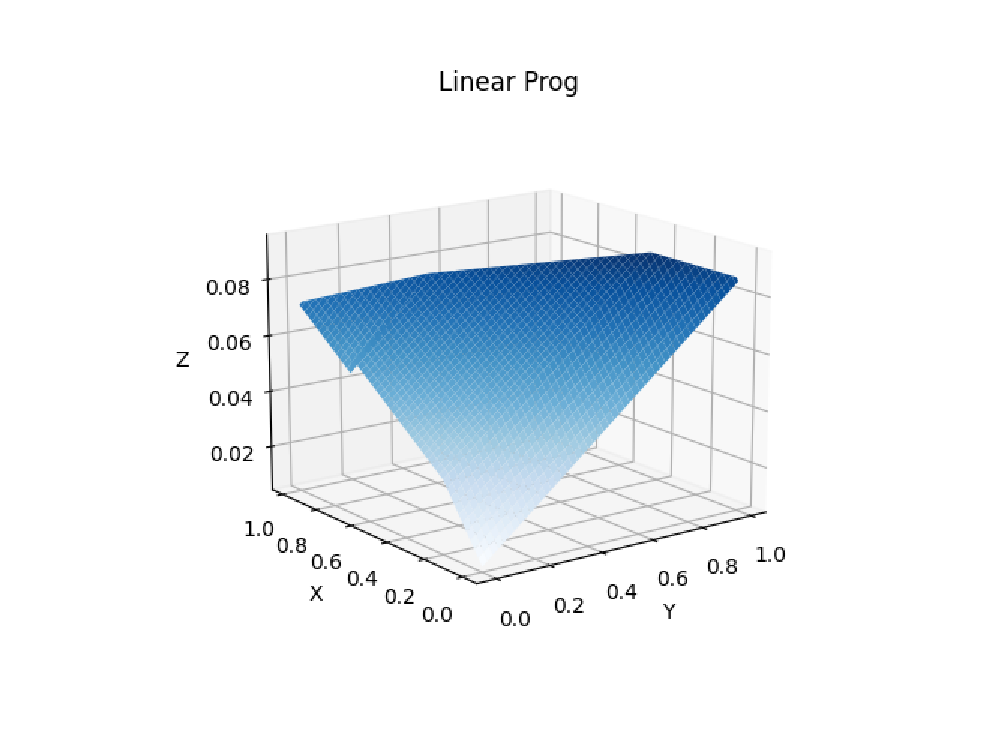
\includegraphics{Figure_1.eps}
				\caption{Линейное программирование}
			\end{figure} 
			
			В целом, использование мягких качественных ограничений при принятии инвестиционных решений заключается в том, чтобы оценить на доле различных финансовых продуктов в неизвестном портфеле, или, рассчитывать, как сильно колебания цен исходных сырей повлияют на цены акций. 
			
			Для первого случая, пусть $r_n$ -- доходность различных финансовых продуктов, $x_i$ -- доля i-го продукта в общем инвестицийб и $z = \min\{r_n(x_{i_n}-x_{j_n})\}$ мы можем построить математическую модель следующим образом:
			\begin{equation*}
				\left\{
				\begin{array}{lr}
					z \sim \displaystyle\max\\
					r_1(x_{i_1}-x_{j_1}) \ge z\\
					\vdots\\
					r_n(x_{i_n}-x_{j_n}) \ge z\\
					\displaystyle\sum_{i=1}^{k}x_i = 1\\
					x_i \ge 0,\quad i = 1,\dots,k
				\end{array}
				\right.
			\end{equation*}
		\subsection{2.2 Решения с нелинейными мягкими ограничениями}
			Если же функции $c_i$ нелинейны, задача \eqref{eq5} может быть решена методом доверительных областей.

\newpage
	\begin{center}
		\section{Заключение}
	\end{center}

	В настоящей работе, дано определение некорректно поставленных обратных задач оценивания, с помощью известной априорной информации установили задачи с мягкими качественными ограничениями. Показано численное определение мягкого унарного отношения на основе теории возможности Ю. П. Пытьева, и исследовали его основные свойства.
	
	В то же время, мы также исследовали линейный и нелинейный случаи мягких ограничений и дали решения для линейного случая с помощью линейного программирования и кратко объяснили того, каковы перспективы его применения в инвестиционной области.
	
	~\\
	
	~\\
	
	~\\
	
	~\\
	
	~\\
	
	~\\
	
	~\\
			
	\small
	\begin{thebibliography}{22}\addtolength{\itemsep}{-4.5ex}
		\bibitem{1}  Пытьев Ю.П. Возможность как альтернатива вероятности. Математические и эмпирические основы, приложения. М: ФИЗМАТЛИТ, 2016. 600 с.\\
		\bibitem{2}  В. А. Зубюк, Численные методы решения некорректно поставленных обратных задач с мягкими качественными ограничениями, Москва, 2020.\\
	\end{thebibliography}
\end{document}




















